\newpage

\section{Coulomb-Nuclear Interference}
\label{sec:coulomb}

\> outline for this section

\> reason for using 90m data
\> different ways of using 1000 and 90m data: combined (democratically), differential (tensions), combined (each DS used where strong)

%----------------------------------------------------------------------------------------------------

\subsection{Theoretical Framework}
\label{sec:cni framework}

In this section the different components of the combined elastic scattering amplitude, already briefly outlined in the introduction, are discussed in more detail. In particular, the Coulomb amplitude (Section~\ref{sec:cni coulomb}), the nuclear amplitude (Section~\ref{sec:cni nuclear}) and their interference (Section~\ref{sec:cni interference}).

%------------------------------------------------------------------
\subsubsection{Coulomb Amplitude}
\label{sec:cni coulomb}
%
The Coulomb amplitude can be calculated from QED (e.g.~Section 3.2 in \cite{block06}), using empirical electric and magnetic form factors of the proton (e.g.~\cite{puckett10}). It can be shown (e.g.~Section 1.3.1 in~\cite{jan_thesis}) that, at low $|t|$, the effect of both form factors can be described by a single function ${\cal F}$. 

\TODO{Add formula}

\TODO{Choice of FF no impact on final results}

%------------------------------------------------------------------
\subsubsection{Nuclear Amplitude}
\label{sec:cni nuclear}
%
Since the nuclear amplitude can presently not be calculated from first principles, its phenomenological description will be discussed.

\vskip3mm
\hbox to\hsize{\bf Modulus\hfil}

The modulus is closely related to the differential cross-section and thus strongly constrained by experimental observations outside the Coulomb and CNI region. Following especially~\cite{8tev-90m}, the modulus for $|t|~\lesssim~0.2$, i.e. well below the diffractive minimum, will be parametrised as:
\begin{equation}
\label{eq:nuc mod}
| {\cal A}^{\rm N}(t) | = a \exp\left( \sum\limits_{n}^{N_b} b_n t^n \right)\ ,
\end{equation}
where $N_b$ gives the number of free parameters in the exponent. This implicitly extends the exponential behaviour to the regions where the (pure nuclear) cross-section cannot be observed. Although there is no rigorous justification, and therefore it stands as an assumption, it is compatible with many theoretical models.

\TODO{considering $N_b = $ 1, 2 and 3 parameters, with more parameters no improvement of $\chi^2$}

\TODO{anchored to $90\un{m}$ data at $|t| > 0.2\un{GeV^2}$ for stability of integrations in Eq.~(\ref{eq:int kl}); high t part has no effect on final results}

\TODO{This parametrisation assumes that Coulomb effects are small, which is not unreasonable, the expected order is few percent}

\vskip3mm
\hbox to\hsize{\bf Phase\hfil}

For the phase of the nuclear amplitude, there is little experimental guidance and therefore several theory-motivated choices will be assumed and tested.

\begin{itemize}
% ***
\item A {\it constant phase} is obviously the simplest choice:
\begin{equation}
\label{eq:nuc phase con}
\arg {\cal A}^{\rm N}(t) = p_0 = \hbox{const.}
\end{equation}
Note that this is equivalent to a strict proportionality of real and imaginary part of the amplitude at all $t$.

% ***
\item The {\it standard phase} parametrisation,
\begin{equation}
\label{eqn:nuc phase std}
\arg {\cal A}^{\rm N}(t) = p_{0} + \arctan \left(\frac{|t|-|t_{0}|}{\tau}\right) -  \arctan \left(\frac{-|t_{0}|}{\tau}\right) \: ,
\end{equation}
implements the main features of many theoretical models -- almost imaginary amplitude in the forward direction ($p_0 \approx \pi/2$) while almost purely real in the (first) diffraction dip. The parameters $t_0 = - 0.50\un{GeV^2}$ and $\tau = 0.1\un{GeV^2}$ have been chosen such that the shape is similar to a number of model predictions, see Figure~\ref{fig:phase illustration}.

% ***
\item Another parametrisation is by {\em Bailly et al.}~\cite{bailly87}:
\begin{equation}
\label{eq:nuc phase bai}
	%\arg {\cal A}^{\rm N}(t) = {\pi\over 2} - \arctan {\rho_0\over 1 - {t\over t_{\rm d}}},\ \rho_0 = {1\over \tan p_0}
	\arg {\cal A}^{\rm N}(t) = \arctan \left[ \tan p_0 \left(1 - {t\over t_{\rm d}} \right) \right]\ ,
\end{equation}
where $p_0$ determines the phase value at $t=0$ and $t_{\rm d} \approx -0.53\un{GeV^2}$ gives the position of the diffractive minimum at $8\un{TeV}$ (preliminary result from $90\un{m}$ data). This phase has behaviour qualitatively similar to the model of Jenskovszky et al., see Figure~\ref{fig:phase illustration}.

% ***
\item The {\it peripheral phase} \cite{kl94} provides an alternative to the above descriptions. Its parametrisation
\begin{equation}
\label{eq:nuc phase per}
\arg {\cal A}^{\rm N}(t) = p_0 - A \exp\left[ \kappa \left( \log {t\over t_{\rm m}} - {t\over t_{\rm m}} + 1 \right) \right]
\end{equation}
%results in a peak at $t_{\rm m} \approx -0.310\un{GeV^2}$, with amplitude $A \approx 5.53$ and width controlled by $\kappa \approx 4.01$.
results in a peak at $t = t_{\rm m}$, with an amplitude $A$ and width controlled by $\kappa \approx 4.01$, as can be seen in Figure~\ref{fig:phase illustration}.
\end{itemize}

\begin{figure*}
\begin{center}
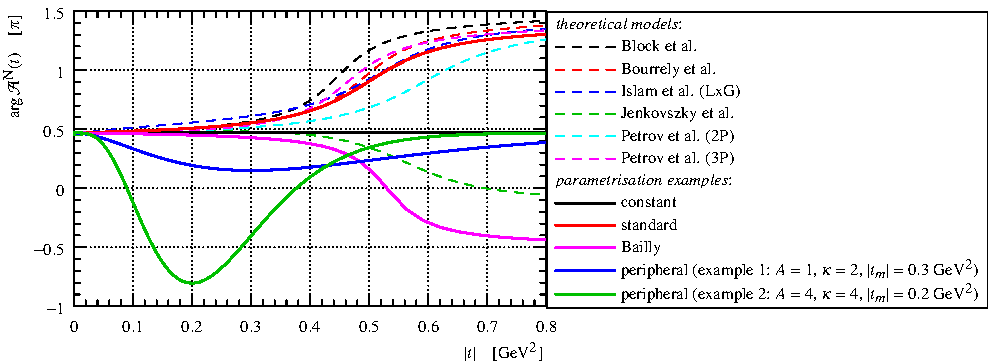
\includegraphics{fig/hadronic_phase_illustration.pdf}
\caption{Illustration of hadronic-phase forms. The dashed lines correspond to predictions by theoretical models as provided by \cite{elegent}. The solid lines give typical examples of parametrisations used in the study, all at the same value of $\rho = 0.10$.
}
\label{fig:phase illustration}
\end{center}
\end{figure*}

Figure~\ref{fig:phase illustration} presents a comparison of phase predictions of several models to typical examples of parametrisations proposed above.

It should be noted that the phase has decisive influence on the amplitude behaviour in the space of impact parameter, $b$, see e.g.~Section 3 in~\cite{klk02}. It can be quantified by evaluating the root-mean-squares (RMS) of $b$ for elastic and inelastic collisions. The constant, standard and Bailly phases lead to elastic collisions more central (smaller RMS) than the inelastic ones. The peripheral phase can yield a description with the opposite hierarchy, which is argued more natural by some authors (e.g. Section~4 in~\cite{kl96}).

%------------------------------------------------------------------
\subsubsection{Coulomb-Nuclear Interference Formulae}
\label{sec:cni interference}

The {\bf simplified West-Yennie formula (SWY)} \cite{wy68} is derived in the framework of perturbative QFT by evaluating the lowest-order Feynman diagrams that comprise both nuclear and Coulomb interactions. In this approach, the interference is reduced to an additional phase between the Coulomb and nuclear amplitudes. Moreover, several approximations were used in the derivation. First, in order to avoid integrating over off-mass-shell contributions to the nuclear amplitude (purely known), very slow variation of the nuclear amplitude phase was assumed: $\arg {\cal A}^{\rm N} \approx \hbox{const}$. Then, in order to obtain a closed-form expression, the exponential slope of the nuclear modulus
\begin{equation}
\label{eq:nuc slope}
B^{\rm N}(t) = {\d \log |{\cal A}^{\rm N}|^2 \over \d t}
\end{equation}
was assumed constant. The original formula did not contain the electromagnetic form factor ${\cal F}$, it was added later by hand:
\begin{equation}
\label{eq:int swy}
	\begin{aligned}
		{\d\sigma\over \d t}^{\rm C+N} &= {\pi (\hbar c)^2 \over s p^2} \left | {\alpha s\over t} {\cal F}^2 \e^{\I\alpha \Phi(t)} + {\cal A}^{\rm N} \right |^2\ ,\cr
		\Phi(t) &= - \left( \log {B^{\rm N} |t|\over 2} + \gamma \right)\ ,\cr
	\end{aligned}
\end{equation}
where $\alpha$ is the fine structure constant and $\gamma \doteq 0.577$ the Euler constant. Despite the many limitations, the formula has extensively been used in past data analyses. For backward-comparison reasons we consider it also in this report.

The {\bf Kundr\' at-Lokaj\' i\v cek formula (KL)} \cite{kl94} was derived in an impact parameter formalism and it is based on the additivity of eikonals. The derivation poses no limitations on nuclear amplitude and the formula naturally incorporates the electromagnetic form-factor. In this treatment, the interference effect goes beyond a single phase, the $\Psi$ quantity is complex, in general:
\begin{equation}
\label{eq:int kl}
	\begin{aligned}
		{\d\sigma\over \d t}^{\rm C+N} &= {\pi (\hbar c)^2 \over s p^2} \left | {\alpha s\over t} {\cal F}^2 + {\cal A}^{\rm N} \e^{\I\alpha \Psi(t)} \right |^2\ ,\cr
		\Psi(t) &= 
			- \int \d t'\, \log {t'\over t} {\d\phantom{t'}\over \d t'} {\cal F}^2(t') \cr
		&\phantom{=} + \int \d t' \left( {{\cal A}^{\rm N}(t') \over {\cal A}^{\rm N}(t)} - 1 \right) { I(t, t')\over 2\pi }
			\ ,\cr
		I(t, t') &= \int_0^{2\pi} \d\phi\ {{\cal F}^2(t'')\over t''}\ , \cr
		t'' &= t + t' + 2\sqrt{t\, t'} \cos\phi\ ,\cr
	\end{aligned}
\end{equation}
where the $t$ integrations go over the entire kinematically allowed region.

For the calculations presented later on the Elegent implementation \cite{elegent} of the formulae will be used, together with the form-factor of Puckett et al.~\cite{puckett10}.

By analysing the formulae Eq.~(\ref{eq:int swy}) and (\ref{eq:int kl}), one can conclude that in the region where the nuclear amplitude dominates ($|t| \gtrsim 0.003\un{GeV^2}$), the effects due to the Coulomb interaction can be proportional either to $\alpha$ or to the ratio ${\cal A}^{\rm C} / {\cal A}^{\rm N}$. In both cases, the magnitude of the interference effects can be expected at a percent level, as shown in Figure~\ref{fig:cni effect}. The figure also shows that the effects at different $|t|$ probe different parts of the hadronic phase: maximum sensitivity to $\rho$ lies at very low $|t|$ while at higher $|t|$ the effects are sensitive to phase values at higher $|t|$. Another observation that one make from the figure is that for constant and standard phase (and can be generalised to Bailly, too) the effects are very similar, rather mild at higher $|t|$. This can be understood from a very limited variation of the phase at low $|t|$, which is the region contributing most to the integral in Eq.~(\ref{eq:int kl}). In contrary, the higher $|t|$ response to peripheral phases can have various forms, often similar to the ``U shape'' of the reconstructed cross-section, see Figures \ref{fig:fits common con} and \ref{fig:fits common per}.



\begin{figure*}
\begin{center}
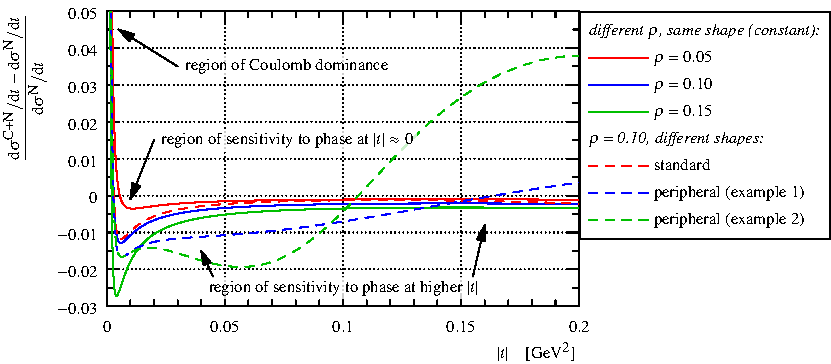
\includegraphics{fig/cni_effect_illustration.pdf}
\caption{%
Illustration of the effects due to the Coulomb interaction, using KL formula. For SWY formula, the picture is similar, however it misses the effects at higher $|t|$. The curves show a response of the interference formula to different nuclear phases with a purely exponential nuclear modulus. The solid curves correspond to phases of the same shape (constant) but different values of $\rho$ (maximal response can be seen at $|t| \lesssim 0.01\un{GeV^2}$). Conversely, the dashed lines correspond to phases with fixed $\rho$ but various shapes (the same examples as in Figure~\ref{fig:phase illustration}), with response sizeable at $|t| \gtrsim 0.02\un{GeV^2}$.
}
\label{fig:cni effect}
\end{center}
\end{figure*}

%----------------------------------------------------------------------------------------------------
\subsection{Fitting/parameter inference}
\label{sec:cni fitting}

%------------------------------------------------------------------
\subsubsection{Task analysis/general discussion}

As indicated in Figure~\ref{fig:cni effect}, in most of the analysed $|t|$ range, the nuclear amplitude dominates. Therefore, it makes sense to think of the complete differential cross-section $\d\sigma^{\rm C+N} / \d t$ as a sum of the nuclear component $\d\sigma^{\rm N} / \d t$ and the effects due to the Coulomb interaction $\d\sigma^{\rm CNI} / \d t$. Now, one could wish to use the measured data (corresponding to $\d\sigma^{\rm C+N} / \d t$) to make statements about the nuclear component only (determine value of $\rho$, $\sigma_{\rm tot}$, etc.). This is, in principle, only possible if the nuclear and CNI components can be separated, for which they would need to be sufficiently distinct. This gives immense weight to the choice of the parametrisations. First of all, the parametrisations set the features that can occur in the nuclear and CNI components and thus also the level of their distinction. For instance, giving too much flexibility to the parametrisations would inevitably make the two components indistinguishable. And even more importantly, the choice of parametrisations has a decisive impact on whether the sum of the two components can be compatible with the data.

Despite the importance of the choice of the parametrisations, there is no rigorous guide (theoretical or any other). This makes the choice (and the following analysis) subjective and to a non-negligible degree arbitrary. Therefore, all the results presented later on will have a character of examples of possible data descriptions. 

\> something about our choice of parametrisations -- ``minimal extensions''
\>> For phase less dramatic -- the form of the CNI component further limited by the KL formula
\>> In modulus parametrisation we implicitly used the fact that CNI is small + unaltered extrapolation to t=0. However, one could imagine more wild descriptions, easily with few percent modification in the parameters of interest.

\>  {\bf conditional} determination of parameters of interest


%------------------------------------------------------------------
\subsubsection{Fitting techniques}

Two alternative objective functions will be used for fitting in this report.

The {\bf standard least squares (LS)} method suggests to minimise
\begin{equation}
\label{eq:chi sq LS}
	\begin{aligned}
		\chi^2 = \vec{\Delta}^\T \mat V^{-1} \vec{\Delta}\ ,\quad \vec{\Delta} &= (\hbox{data} - \hbox{fit})\ ,\cr
																		\mat V &= \mat V_{\rm stat} + \mat V_{\rm syst}\ ,\cr
	\end{aligned}
\end{equation}
where $\vec\Delta$ represents vector of differences in $\d\sigma/\d t$ between fit function and measurement for each point. The covariance matrix $\mat V$ is given by the sum of the statistical component $\mat V_{\rm stat}$ (diagonal) and the systematic component $\mat V_{\rm syst}$.

Later on, different combinations of $\beta^* = 90$ and $1000\un{m}$ data will be used. For the former, the data and uncertainties can be found in Table 3 in \cite{8tev-90m}. For the latter, the data and statistical uncertainties can be found in Table~\ref{tab:data} and the systematic covariance matrix can be calculated by Eq.~(\ref{eq:covar mat}). When both data sets are used, the normalisation uncertainty is treated as fully correlated (normalisation has been deduced from the same reference measurement \cite{prl111}).

\> {\bf Parameter-comparison} method
\>> manifestly binning-independent
\>> can cut off modes with no sensitivity -- strengthening of performance
\>> chi square behaviour, number of degrees of freedom

\begin{equation}
\label{eq:chi sq parcmp}
\chi_{\rm p}^2 = \Delta_{\rm p}^\T \mat V_{\rm p}^{-1} \Delta_{\rm p}\ ,\quad \Delta_{\rm p} = \TODO{...} 
\end{equation}

\> fit quality measures: $\chi^2/ndf$, p-value, significance

%----------------------------------------------------------------------------------------------------
\subsection{Common fits of 1000 and 90m data}

In this section we present results for fit where the $1000$ and $90\un{m}$ data act in equal manner. Technically, the vector $\Delta$ in Eq.~(\ref{eq:chi sq LS}) consists of two sub-columns, one from each data sets.

Figure \ref{fig:fits common con} shows the fit results for the constant nuclear phase. The free parameters include: $a$ and $b_n$ in Eq.~(\ref{eq:nuc mod}) and $p_0$ in Eq.~(\ref{eq:nuc phase con}). One can observe that the standard LS and parameter-comparison fits give very similar results (up to a small difference in normalisation). Therefore, only the parameter-comparison method will be presented in what follows (as it has better sensitivity in addition). Similarly, for $N_b = 1$ the fits with SWY and KL interference formulae are almost identical, thus only KL will be used later on. Still for $N_b = 1$, note the very bad fit quality: more than $7\un{\sigma}$ for the standard LS and almost $10\un{\sigma}$ for the parameter-comparison method. Consequently, one may conclude that the combination of purely exponential nuclear modulus and constant phase is excluded by the data. Moreover, since this is the only combination theoretically compatible with the SWY interference formula, the formula is excluded, too.

Furthermore, as it could be expected from Figure~\ref{fig:cni effect}, the fits with constant, standard and Bailly nuclear phases are nearly identical. Therefore, the constant phase will be used hereafter to represent this group.

%\> Figure \ref{fig:fits common con}
%\>> std LS and par cmp fits very similar (up to small difference in normalisation), can be generalised to all results hereafter
%\>> $N_b = 1$ fits with KL and SWY almost identical (also true in what follows, will use KL to represent both)
%\>> case $N_b = 1$ + constant phase excluded by both fit techniques
%\>>> the only compatible with SWY $\Rightarrow$ SWY excluded, too
%\>> addition (not shown): results for standard and Bailly phase (almost) indistinguishable from the constant one, will use only constant to represent this ``family''

\begin{figure*}
\begin{center}
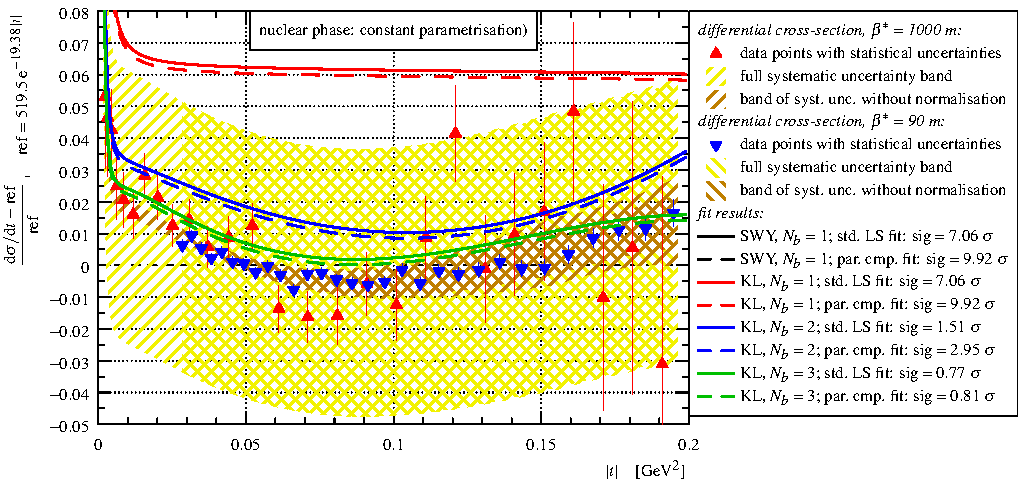
\includegraphics{fig/fits_common_con.pdf}
\caption{%
Fit results for fits with constant nuclear phase, Eq.~(\ref{eq:nuc phase con}). The vertical axis gives the cross-section difference from a reference exponential. The red (blue) triangles represent the $\beta^* = 1000$ ($90\un{m}$) data with their statistical uncertainties. The systematic uncertainties are represented by the hatched bands: yellow (full uncertainty), brown (all systematic uncertainties except for normalisation). The orientation of the hatching indicates the respective data set.
The curves represent fit results obtained with different parametrisations and fit techniques. The solid curves represent standard least-squares fits, the dashed ones fits with the parameter-comparison method. Different colours stand for different interference formulae (SWY/KL) and numbers of parameters in the nuclear modulus exponent, $N_b$, cf.~Eq.~(\ref{eq:nuc mod}). The red curves almost fully cover the black ones.
}
\label{fig:fits common con}
\end{center}
\end{figure*}

Figure \ref{fig:fits common per} shows the fit results for the constant nuclear phase. The free parameters include: $a$ and $b_n$ in Eq.~(\ref{eq:nuc mod}) and $p_0$, $A$, $\kappa$ and $t_m$ in Eq.~(\ref{eq:nuc phase per}). Again, one may conclude that the standard LS fits are very similar to those from the parameter-comparison method (up to a small difference in normalisation for $N_b = 1$). In contrast to the fits with constant nuclear phase, here all the fits have reasonable quality.

\begin{figure*}
\begin{center}
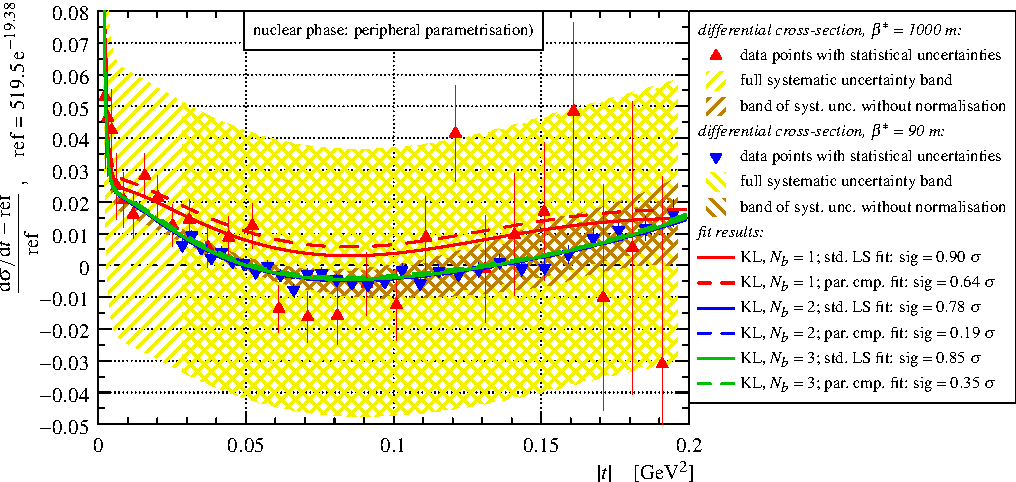
\includegraphics{fig/fits_common_per.pdf}
\caption{%
Fit results for fits with peripheral nuclear phase, Eq.~(\ref{eq:nuc phase per}). Legend identical as in Figure~\ref{fig:fits common con}.
}
\label{fig:fits common per}
\end{center}
\end{figure*}


From the fits presented in Figures~\ref{fig:fits common con} and \ref{fig:fits common per} one may derive parameters of interest related to the nuclear component. In particular $\rho$, exponential slope $B^{\rm N}$ (see Eq.~(\ref{eq:nuc slope})) and the total cross-section via the optical theorem:
\begin{equation}
\label{eq:si tot}
\sigma_{\rm tot}^2 = {16\pi\, (\hbar c)^2\over 1 + \rho^2}\, \left. \d\sigma^{\rm N}\over\d t\right|_0
		= {16\pi^2\, (\hbar c)^4\over s p^2 (1+\rho^2)}\, a^2\ ,
\end{equation}
where $a$ is the intercept of the nuclear modulus parametrisation, cf.~Eq.~(\ref{eq:nuc mod}). The results are given in Table \ref{tab:fits common} and visualised in Figure~\ref{fig:fits reciprocal der} (black points).
\TODO{trends in data? Explain!}
\TODO{comparison to previous measurements, COMPETE extrapolation}
\TODO{illustrative decomposition of uncertainties from MC}

In addition, Table \ref{tab:fits common} gives RMS values of impact parameter $b$ for elastic and inelastic collisions. These parameters quantify the character of the collisions in the impact parameter space and have been calculated according to Section 3 in~\cite{klk02} directly from $t$-space quantities. \TODO{equation??}
One can conclude that irrespectively on $N_b$, the constant-phase fits have central character: elastic collisions occur at smaller impact parameters than the inelastic collisions. In contrary, all the fits with the peripheral nuclear phase lead to opposite (peripheral) hierarchy.


\begin{table*}
\caption{%
Parameters derived from the parameter-comparison fits presented in Figures~\ref{fig:fits common con} and \ref{fig:fits common per}. The rows correspond to different numbers of parameters in the nuclear modulus exponent. The left-hand (right-hand) side columns refer to fits with constant, Eq.~(\ref{eq:nuc phase con}), (peripheral, Eq.~\ref{eq:nuc phase per}) nuclear phase. The RMS values of impact parameter $b$ correspond to elastic (el), inelastic (inel) and any (tot) collisions.
}%
\vskip-3mm
\label{tab:fits common}
\begin{center}
\small
\setlength{\tabcolsep}{5pt}
%\def\arraystretch{0.8}
\begin{tabular}{c@{\hskip20pt}cc@{\hskip20pt}cc}
\hline
\hline
% header
	& \multispan2\hfil constant \hfil & \multispan2\hfil peripheral \hfil  \cr
\hline
 			& $\rho = -0.027 \pm 0.021$ & $\sqrt{\langle b^2\rangle_{\rm el}} = 0.87\un{fm}$					& $\rho = 0.083 \pm 0.023$ & $\sqrt{\langle b^2\rangle_{\rm el}} = 1.68\un{fm}$					\cr
$N_b = 1$	& $B = (19.39 \pm 0.05)\un{GeV^{-2}}$ & $\sqrt{\langle b^2\rangle_{\rm inel}} = 1.34\un{fm}$		& $B = (19.68 \pm 0.07)\un{GeV^{-2}}$ & $\sqrt{\langle b^2\rangle_{\rm inel}} = 1.03\un{fm}$		\cr
			& $\sigma_{\rm tot} = (103.8 \pm 2.1)\un{mb}$ & $\sqrt{\langle b^2\rangle_{\rm tot}} = 1.23\un{fm}$	& $\sigma_{\rm tot} = (102.8 \pm 2.1)\un{mb}$ & $\sqrt{\langle b^2\rangle_{\rm tot}} = 1.24\un{fm}$	\cr\hline
%                                                                                                                                                                                                                   
 			& $\rho = 0.059 \pm 0.021$ & $\sqrt{\langle b^2\rangle_{\rm el}} = 0.87\un{fm}$						& $\rho = 0.120 \pm 0.026$ & $\sqrt{\langle b^2\rangle_{\rm el}} = 1.90\un{fm}$						\cr
$N_b = 2$	& $B = (19.97 \pm 0.07)\un{GeV^{-2}}$ & $\sqrt{\langle b^2\rangle_{\rm inel}} = 1.36\un{fm}$		& $B = (20.46 \pm 0.44)\un{GeV^{-2}}$ & $\sqrt{\langle b^2\rangle_{\rm inel}} = 0.96\un{fm}$		\cr
			& $\sigma_{\rm tot} = (102.8 \pm 2.1)\un{mb}$ & $\sqrt{\langle b^2\rangle_{\rm tot}} = 1.25\un{fm}$	& $\sigma_{\rm tot} = (104.13 \pm 2.3)\un{mb}$ & $\sqrt{\langle b^2\rangle_{\rm tot}} = 1.28\un{fm}$	\cr\hline
%                                                                                                                                                                                                                   
 			& $\rho = 0.090 \pm 0.024$ & $\sqrt{\langle b^2\rangle_{\rm el}} = 0.87\un{fm}$						& $\rho = 0.115 \pm 0.026$ & $\sqrt{\langle b^2\rangle_{\rm el}} = 2.01\un{fm}$						\cr
$N_b = 3$	& $B = (20.39 \pm 0.14)\un{GeV^{-2}}$ & $\sqrt{\langle b^2\rangle_{\rm inel}} = 1.37\un{fm}$		& $B = (20.04 \pm 0.36)\un{GeV^{-2}}$ & $\sqrt{\langle b^2\rangle_{\rm inel}} = 0.82\un{fm}$		\cr
			& $\sigma_{\rm tot} = (102.5 \pm 2.1)\un{mb}$ & $\sqrt{\langle b^2\rangle_{\rm tot}} = 1.26\un{fm}$	& $\sigma_{\rm tot} = (103.5 \pm 2.2)\un{mb}$ & $\sqrt{\langle b^2\rangle_{\rm tot}} = 1.25\un{fm}$	\cr\hline
\hline
\end{tabular}
\end{center}
%\vskip-10mm
\end{table*}



%----------------------------------------------------------------------------------------------------
\subsection{Reciprocally constrained 1000 and 90m fits}


\begin{figure*}
\begin{center}
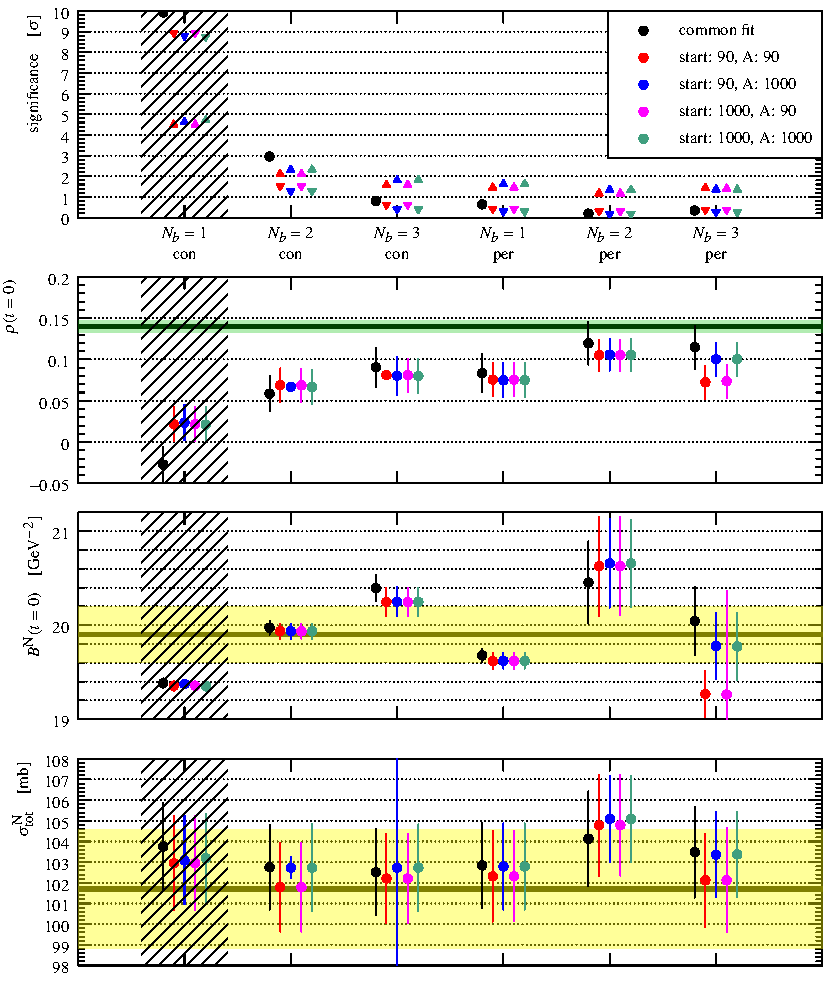
\includegraphics{fig/fits_reciprocal_derived.pdf}
\caption{\TODO{caption}
Points as in legend, black ones correspond to the results of Table~\ref{tab:fits common}. Significance: triangles up (down) from 1000m (90m) fit. Describe columns -- combinations of $N_b$ and phase parametrisation. The column $N_b=1$ and constant phase is hatched since this combination is excluded by the data. Yellow horizontal bands: results from PRL, reference to the delicate B comparison above? Green horizontal band: extrapolation by COMPETE - which one? Peripheral fits -- shape variable or fixed?
}
\label{fig:fits reciprocal der}
\end{center}
\end{figure*}
